%tag:000X
%label:"fig:handleslide"
%author:JeffHicks
%name:"handleslide"
%type:"figure"
%parent:def:heegaardMoves
%caption:"The cycles \(\alpha_{g-1}, \alpha_g\)and \(\alpha_g'\) are related by handleslide"



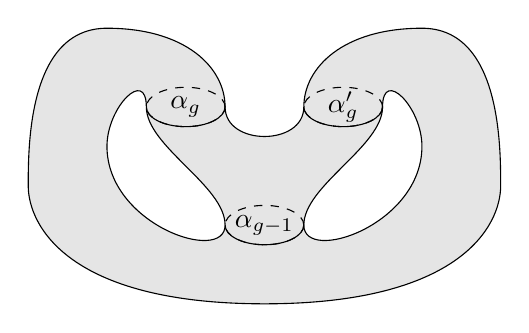
\begin{tikzpicture}





    \draw[fill=gray!20] (-0.5,1.5) .. controls (-1.5,1.5) and (-1.5,0) .. (-1.5,-0.5) .. controls (-1.5,-1) and (-1,-2) .. (1.5,-2) .. controls (4,-2) and  (4.5,-1) .. (4.5,-0.5) .. controls (4.5,0) and (4.5,1.5) .. (3.5,1.5) .. controls (2.5,1.5) and (2,1) .. (2,0.5) .. controls (2,0) and (1,0) .. (1,0.5) .. controls (1,1) and (0.5,1.5) .. (-0.5,1.5);
    \begin{scope}[]
    \draw[fill=white] (0,0.5) .. controls (0,1) and (-0.5,0.5) .. (-0.5,0) .. controls (-0.5,-1) and (1,-1.5) .. (1,-1) .. controls (1,-0.5) and (0,0) .. (0,0.5);
    
    \end{scope}
    \begin{scope}[xscale=-1, shift={(-3,0)}]
    \draw[fill=white] (0,0.5) .. controls (0,1) and (-0.5,0.5) .. (-0.5,0) .. controls (-0.5,-1) and (1,-1.5) .. (1,-1) .. controls (1,-0.5) and (0,0) .. (0,0.5);
    
    \end{scope}
    
    
    \begin{scope}[shift={(1,1.5)}]
    \draw[dashed]  (1.5,-1) ellipse (0.5 and 0.25);
    \clip  (2,-1) rectangle (1,-1.75);
    \draw  (1.5,-1) ellipse (0.5 and 0.25);
    \end{scope}
    
    
    \begin{scope}[shift={(0,0)}]
    \draw[dashed]  (1.5,-1) ellipse (0.5 and 0.25);
    \clip  (2,-1) rectangle (1,-1.75);
    \draw  (1.5,-1) ellipse (0.5 and 0.25);
    \end{scope}
    
    
    \begin{scope}[shift={(-1,1.5)}]
    \draw[dashed]  (1.5,-1) ellipse (0.5 and 0.25);
    \clip  (2,-1) rectangle (1,-1.75);
    \draw  (1.5,-1) ellipse (0.5 and 0.25);
    \end{scope}
    
    \node at (1.5,-1) {$\alpha_{g-1}$};
    \node at (0.5,0.5) {$\alpha_g$};
    \node at (2.5,0.5) {$\alpha_g'$};
    \end{tikzpicture}